%PUT STG, COG, ADG as option
\documentclass[COG,11pt]{ercgrant}
% put here the year of the call
\renewcommand{\callyear}{2023}
% \setmainfont{Arial}
\bibliography{bibliography.bib}
% \bibliography{nature-refs.bib}

\newcommand{\oonetitle}{An video-driven digital twin of mouse visual cortex during free behavior}
\newcommand{\otwotitle}{Find tuning changes and characterize uncertainty in latent dimensions}
\newcommand{\othreetitle}{Identify causal links between neural representations and behavior}
\author{Fabian Sinz}
\acro{Visual System in Action}
% \title{Putting data-driven digital twins of mouse visual cortex into action.}
% \title{Towards a meta-verse for the mouse visual system}
% \title{Building a data driven model how behavior changes neuronal processing in mouse visual cortex in freely behaving mice}
\title{A data-driven characterization of free behavior's impact on mouse visual processing}
\institution{Georg August Universität Göttingen Stiftung Öffentlichen Rechts}


% ====== BODY OF THE DOCUMENT ======
\begin{document}

\maketitle

% \begin{abstract}
% \end{abstract}
\begin{mdframed}
Sensory systems are our window to the world and form the basis for our decisions and behavior. 
However, sensory processing is not a one-way street:
Motor behavior and the internal state of an animal can alter how sensory signals are processed.
Even in head-restrained animals, previous studies found a rich influence of motor behavior on neural activity. 
How and when the brain adjusts sensory processing during unconfined real-world  behavior in complex natural environments is currently unknown. 
I hypothesize that, under these conditions, the brain dynamically adjusts sensory processing to the current behavioral context not only by changing the gain, but the selectivity of sensory neurons. 
I further hypothesize that these changes momentarily increase the reliability of relevant environmental aspects in neuronal representations. 

I will investigate this in the visual system of mice by building deep data-driven functional twin models of visual cortex and behavior in digital replicas of real experimental environments.
The models will be trained on a massive dataset of recordings from excitatory neurons from nine areas of visual cortex in head-fixed and freely behaving mice under spontaneous and task-driven behavior.
I will use these twins to discover which neurons change their tuning, how and under which behavioral context they change it, and how the animal's behavior would be different if these mechanisms were shut down.
If successful, this project will not only change our view on how the visual system adapts to behavior under natural conditions, but also yield a computational framework with a vast range of applications in neuroscience. 
It is straightforward to generalize to other areas, stimulus modalities, and species, and will be an enabling tool to study how the brain makes sense of the environment in unconfined behaving animals.

% in real world tasks
 % -- not only changing the gain, but also the selectivity of single sensory neurons
\end{mdframed}

%%%%%%%%%%%%% EXTENDED SYNOPSIS %%%%%%%%%%%%%%%%%%%

\section{Extended Synopsis of the Scientific Proposal}

\subsection{Background, state of the art and rationale}
The goal of the visual system is to extract actionable information about our environment from the complex and ambiguous light patterns that inform our brain about the world beyond our eyes.
But vision is not a one-way street: The activity of each neuron in the visual system is not only determined by visual input, but also changes with the internal or behavioral state of the animal~\parencite{Niell2010-bs, Erisken2014-un, Reimer2014-cf, Busse2017-rt, Musall2019-kd, Franke2022-do}. 
However, almost all previous work regarding the influence of behavior on the representation of visual stimuli have been performed in head-fixed animals using simple stimuli.
Consequently, when and how visual representations of complex natural stimuli adapt to behavioral context in freely viewing and behaving animals is unknown. 
The goal of this proposal is to investigate the hypothesis that
\textbf{neurons in mouse visual cortex adapt their stimulus preference to the current  motor behavior to decrease uncertainty about momentarily relevant aspects of the world. To test this hypothesis, I will build a computational framework based on data-driven deep neural network models of the visual system, detailed motor behavior captured by posture graph trajectories of freely behaving mice, scanned virtual replicas of experimental` environments, and reinforcement learning.}

Why would the brain adapt sensory representations? When actions need to be chosen on the basis of uncertain sensory information about the world, decreasing uncertainty about relevant aspects for the current behavioral goal becomes imperative~\parencite{Chebolu2022-tb}. 
If this comes at a cost -- energy or opportunity --, it makes sense to selectively adapt visual processing to the behavioral context, \eg~focusing on  higher temporal frequencies while the animal is walking, running, or flying.
Decades of research in head-restrained animals watching simple stimuli such as bars, dots, and gratings have demonstrated that visual processing is modulated by both motor activity and the internal state of the animal~\parencite{Rowell1971-zj, Wiersma1968-xt, Motter1993-od, Maimon2010-sa, Niell2010-bs,Bezdudnaya2006-ge, Treue1996-lp, Musall2019-kd, Busse2017-rt}, and can result in better behavioral performance \parencite{Spitzer1988-kq, Bennett2013-rk, Dadarlat2017-jw, De_Gee2022-ir}.
In many cases, state-dependent modulation has been reported to  affect neural responsiveness, called \textit{gain} \parencite{Eggermann2014-xp, Niell2010-bs, McAdams1999-cs,Schroder2020-jl, Dadarlat2017-jw, Mineault2016-fk}. 
In other cases, the stimulus preference of sensory neurons itself changes \parencite{Chiappe2010-bm, Bezdudnaya2006-ge, Andermann2011-vw, Treue1996-lp}. 
Using more ethological UV-color stimuli and data-driven deep network models, we recently showed that arousal -- correlated with a dilated pupil and running -- can change stimulus selectivity of neurons in mouse visual cortex at the timescale of seconds~\parencite{Franke2022-do}. 
\textcite{Stringer2019-lt} recently showed that spontaneous neuronal population activity is modulated by multi-dimensional latent fluctuations, related to detailed motor activity of the animal~\parencite{Syeda2022-bk}.
Using auditory and visual decision making tasks, \textcite{Musall2019-kd} found that task-irrelevant motor behavior becomes increasingly locked to the task and strongly modulates neuronal activity.
These studies demonstrate that -- even in head-fixed animals -- activity in visual cortex and other sensory areas is heavily influenced by motor activity, promising an even richer repertoire of how behavior can affect visual processing in freely moving animals in complex environments~\parencite{Busse2017-rt,Huk2018-ez, Datta2019-qj}.
However, a detailed understanding \textit{which} neurons change their selectivity under natural conditions, \textit{how} they change it, and in \textit{which behavioral context} is currently missing.


Fortunately, addressing these questions comes within reach as recent years have seen a paradigm shift towards tracking detailed behavior and recording neuronal activity in freely moving animals~\parencite{Wallace2013-lf,Del_Grosso2017-ww,Mathis2018-lk,Cai2016-rh, Parker2022-ac}.
But extracting meaningful insights from these data poses new computational challenges:
\circled[gray][gray][white]{1} To understand the interaction of visual processing and behavior, we need to disentangle the contributions of the stimulus, the behavior, and the internal state of the animal to the activity of neurons during free behavior. 
This includes reconstructing what the animal saw at every moment of the experiment, and developing models that can capture common fluctuations due to motor behavior or internal state in the neuronal population activity.
\circled[gray][gray][white]{2} To characterize how stimulus selectivity changes with behavior in a classical experimental trial structure, one would need to present the same stimuli in different behavioral contexts. 
However, behavior and visual input in natural conditions cannot easily be controlled or repeated, and natural stimuli are not easily parametrized.
\circled[gray][gray][white]{3} To derive new predictions and experimental paradigms, we need a computational framework that allows us to simulate conditions not found in the experimental recordings, and to possibly perform experimentally impossible manipulations~\parencite{Walker2019-yw, Franke2022-do,Bashivan2019-ry}. Existing work on visual responses during free behavior uses linear techniques, such as generalized linear models, are not suited to address the above challenges.

To fill this gap, I will develop a new computational framework that can compile behavioral and physiological observations (across multiple experiments) into a single computational model -- a \textbf{functional twin}\footnote{I will use the term \textit{functional twin} for a model that can faithfully predict measurable observations for a real system, such as neural activity or behavior, over a large range of conditions, \eg~arbitrary videos or behaviors. A functional twin mimics the system \textit{functionally}, without necessarily resembling it \textit{structurally}.}. It will allow me to efficiently explore the neuronal response functions across the joint space of stimuli and behavior \textit{in silico}, and in turn make specific predictions that are testable \textit{in vivo}.
This functional twin will be based on data-driven deep network models of neuronal activity and behavior in scanned virtual replicas of the real experimental environment (Fig.~\ref{fig:replica}).
In the last years, we~\parencite{Walker2019-yw, Cobos2022-rr, Franke2022-do} and others~\parencite{Bashivan2019-ry, Ponce2019-yn, Hofling2022-wr} have shown that deep artificial neural networks (ANNs) can learn highly predictive models of complex neuronal representations from data of multiple experiments and can generate new, experimentally testable insights.
My team and I have demonstrated that these models can extract characteristic features of visual cortex that generalize across stimuli, neurons, and animals~\parencite{Sinz2018-sk,Lurz2020-ua,Cobos2022-rr}, and can extract meaningful internal states from large scale population recordings~\parencite{Bashiri2021-or}. 
Using these models, we have found novel stimulus selectivities in  mouse primary visual cortex~\parencite{Walker2019-yw,Franke2022-do} that substantially deviate from previous text book knowledge~\parencite{Hubel1959-zs}.
Models based on our network architectures are currently state of the art in predicting neuronal activity in mouse visual cortex\footnote{All winners of  \url{https://sensorium2022.net/} used our base network architecture}. 
In fact, the authors of the \textit{neuroconnectionist research programme}~\parencite{Doerig2022-ex} advocated for ANNs as ``a computational language for expressing falsifiable theories about brain computation'' to generate ``new and otherwise unreachable insights''. 
Extending them by motor behavior and embedding them in scanned virtual replicas of real environments will not only allow me to study the effect of free motor behavior on visual processing, but also create a widely applicable, unified computational framework to study sensory neuroscience in freely behaving animals. 





\subsection{Objectives}
\begin{wrapfigure}[10]{R}{.20\textwidth}
\vspace{-4ex}
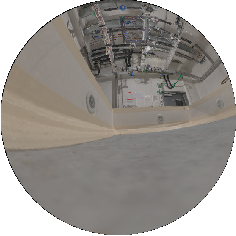
\includegraphics[width=\linewidth]{figures/rendered.pdf}
\caption{\textbf{Rendered} mouse view in virtual replica~\parencite[from][]{Holmgren2021-jv}.}
\label{fig:replica}
\end{wrapfigure}
I propose to build a functional twin of mouse visual cortex and behavior by merging a deep video-based model of stimulus-driven and latent neuronal activity in visual cortex with detailed behavior captured by trajectories of posture graphs. The model will be trained on a massive dataset of visual responses and behavior, shared with me by two long-term collaborators. I will place this model in LIDAR-scanned virtual replicas of real experimental environments (see Fig.~\ref{fig:replica}) and replay visual input and behavior from actual or simulated experiments to the model.
% such that changes of visual computations with behavior and internal state are preserved. 
This framework allows me to discover novel ways \textit{how} neuronal selectivity  changes during spontaneous and goal-driven behavior, and investigate \textit{why} the visual system exhibits these changes by predicting how disabling them affects task-performance and behavior. The project is structured into three objectives:

\obj{1} \textbf{\oonetitle} to \textbf{disambiguate the contributions of stimulus, behavior, and internal state} to neuronal responses in miniscope recordings~\parencite[see Fig.~\ref{fig:miniscope}]{Cai2016-rh} of freely moving animals. This model will form the backbone for \obj{2} and \obj{3}.

\obj{2} \textbf{\otwotitle} in the model and quantify which scene properties are represented more reliably as a result by reconstructing 3D scene properties from the model. This addresses \textit{how} selectivity changes with behavior, and what this means in terms of stimulus representation. 
% I expect a close correspondence between motifs of motor behavior and which scene aspects are more accurately represented. 

\obj{3} \textbf{\othreetitle} by training the functional twin how to solve an open field object recognition task (Fig.~\ref{fig:openfield}) in the virtual environment and observing the effect of circuit manipulations in the model on the twin's behavior. 
This investigates \textit{why} selectivity changes with behavior.


\subsection{Significance}

\textbf{Beyond state of the art \& potential impact.} 
I will develop essential computational technology to step away from the typical trial-based structure of systems and behavioral neuroscience, and to enable a ``natural neuroscience'' in unrestrained animals under complex natural conditions that are not easily controlled or repeated. 
If successful, it will not only change our view on how free behavior affects the visual system, but also yield a computational framework that pushes multiple boundaries in neuronal data science and has countless applications beyond this project:
\circled[black][black][white]{1} It will be the first unified model to capture how free behavior affects stimulus selectivity of real neurons in visual cortex. 
It offers the possibility to include other areas (such as motor or prefrontal areas), or stimulus modalities (such as sound or proprioreception), or more detailed observations (such as whisking or biophysical body models). 
\circled[black][black][white]{2} Embedding it into virtual replicas of real environments, instead of directly recording the visual input to the mouse during experiments~\parencite{Parker2022-ac}, allows me to predict the activity of real neurons to entirely new behaviors. 
\circled[black][black][white]{3} Using reinforcement learning in combination with models of visual cortex for predicting changes in free behavior under causal manipulations of the circuit is unprecedented, and offers an innovative way to bridge the gap between visual representations and behavior. 
The framework is readily generalizable to other tasks and questions, even  pharmacological interventions, and will be a powerful tool to make specific predictions about how changes in sensory representations affect behavior.
As the volume, detail, and complexity of neuroscience data is increasing, the proposed approach is one step towards a \textit{standard model of systems neuroscience}.
The framework will not replace experiments, but make it easier, faster, and cheaper to generate specific predictions \textit{in silico} before testing them \textit{in vivo}.


\begin{wrapfigure}[10]{R}{.30\textwidth}
\vspace{-1.8ex}
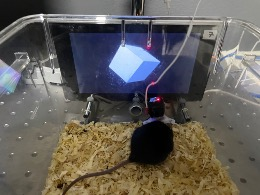
\includegraphics[width=\linewidth,trim=25 15 10 30, clip]{figures/miniscope.jpg}
\caption{Mouse with miniscope in task arena of Dr. Froudarakis.}
\label{fig:miniscope}
\end{wrapfigure}
\textbf{Interdisciplinarity and data resources.} In this project, I will develop novel machine learning methods for fundamental research questions in neuroscience. Such a project requires strong expertise in both fields. 
I am trained in bioinformatics (undergraduate), machine learning (since undergraduate), computational neuroscience (PhD), and neuroscience (postdoc). 
I was the coordinator for machine learning and computational neuroscience in a large consortium\footnote{Machine Intelligence from Cortical Networks: \url{https://ninai.org}; see \nameref{sec:trackrecord}} to understand the cortical algorithms of vision.
This and multiple follow-up projects give me access to >18M neuron-hours of responses to visual stimuli across nine areas of mouse visual cortex recorded with widefield 2-photon microscopes~\parencite{Sofroniew2016-xg} in the lab of my long-term collaborator Dr.~Tolias (Baylor College of Medicine, Houston, co-author on >20  publications). In addition, my long-time collaborator Dr. Froudarakis (FORTH, Crete, co-author on >10 publications) 
% and Dr. Tolias (Baylor College of Medicine, Houston, co-author on >20  publications) 
will share with me behavioral videos and neuronal responses, recorded with miniscopes~\parencite[Fig~\ref{fig:miniscope}]{Cai2016-rh} in freely behaving mice during spontaneous or task-driven behavior.
The animals perform open field visual object recognition tasks (Figs~\ref{fig:openfield}). Dr. Froudarakis will also share data from visual cortex of head-fixed and freely behaving mice under optogenetic suppression of different visual areas with me. Dr. Froudarakis is recording this data for other ongoing grants. My framework is not required for these grants, but opens new possibilities to analyze their data.
Both also agreed to run supplementary experiments to test our predictions.



% computational goal also unclear for mid -level areas
% \subsection{Objective details}
% \newcommand{\itbf}[1]{\textit{\textbf{#1}}}



\subsubsection{Objective 1: \oonetitle~(4 yrs, PhD1, PD)\hfill\obj{1}}
\labelobj{1}
\underline{Goal:} Build a model for neuronal activity in visual cortex of behaving mice to disambiguate the contributions of stimulus, behavior, and internal state to neuronal responses. 

% % \itbf{Significance:} The model is general and can be used to predict neuronal responses for novel visual input and behavior. It thus forms a general computational framework to address questions in sensory neuroscience and behavior beyond this proposal. Here, it will form the backbone for the analyses in \obj{2} and \obj{3}.

\underline{Overview and rationale:}
I will build on my pioneering work on deep data-driven models for visual cortex on video-~\parencite{Sinz2018-sk} and image-based latent state models~\parencite{Bashiri2021-or}, and pre-train a deep video-driven latent state model of visual cortex on responses of $>100,000$ neurons from nine areas of visual cortex recorded in head-fixed mice.
Based on previous work~\parencite{Stringer2019-lt}, I expect the latent activity to be low dimensional compared to the number of neurons which will allow me to identify most of the latent space from head-fixed experiments and fine-tune it on experiments from freely behaving animals. 
We previously demonstrated that pre-training data-driven models allows for an efficient generalization to new neurons and mice~\parencite{Lurz2020-ua} which will foster a quick adaptation to recordings from free behavior. 
We will transfer this model to the viewpoint of freely behaving mice to model neuronal responses recorded with a miniscope~\parencite{Cadena2017-rb}.
We will generate the visual input by replaying the mouse behavior in a virtual replica of the experimental environment and rendering environment from the mouse's point of view. 
This will also allow us to simulate a visual system with many more neurons from the point of view of the behaving animal.
To model the effect of behavior on neuronal selectivity, we will include the tracked posture graph of the animals in the model and use it to explain changes in the neuronal representations.


\underline{Approach:} 
The architecture of the video-driven latent state model will be based on two of my previous works: It will use a common feature space, represented by a convolutional recurrent network~\parencite{Sinz2018-sk}, and a shared latent space~\parencite{Bashiri2021-or}. 
To capture behavior, we will extract the movement of the mouse using 2D keypoints of its posture graph~\parencite{Mathis2018-lk}. 
We will transfer it to 3D using triangulation and lifting  with an algorithm we developed that can deal with temporarily occluded keypoints~\parencite{Pierzchlewicz2022-tq}. 
To model visual input from arbitrary viewpoints, we will build a virtual replica of the experimental environment (Fig.~\ref{fig:miniscope}) using LIDAR scanning and baking images of the environment as texture onto the scanned mesh~\parencite[Fig.~\ref{fig:replica}]{Holmgren2021-jv}. 
We will embed the stimulus screen in the environment using Blender.
% Since the cage and lab environment are standardized and static, we can do that for existing scans in hindsight.
To build the functional twin, we will place a camera at the approximate eye locations of the mouse and move it in the digitized environment according to the movement of the mouse. 
The rendered frames will yield the input to the video-driven model.
We will then freeze the weights of the visual model and learn simple readouts to predict neuronal activity of the miniscope recordings.
We will fine-tune the location of the eye using known compensatory eye movements of the mouse~\parencite{Wallace2013-lf} and adjust the gaze position based on pupil position from an eye camera by maximizing the predictive accuracy for neuronal activity~\parencite[similar to][]{Sinz2018-sk, Parker2022-ac}.
The posture graph trajectories will serve as additional input, bias the latent state and result in a change of stimulus selectivity. 

\underline{Expected outcome:} A functional twin that can faithfully predict neuronal activity from miniscope recordings of freely behaving mice in terms of visual input, motor behavior, and internal state.

%----------------------------------------------------------
\subsubsection{Objective 2:  \otwotitle~(4 yrs, PhD2)\hfill\obj{2}}
\labelobj{2}
\underline{Goal:} Find the correspondence between behavioral context and changes in stimulus selectivity, and how they affect uncertainty about semantic and geometric scene properties. 

\begin{wrapfigure}[5]{r}{.4\textwidth}
\vspace{-2ex}
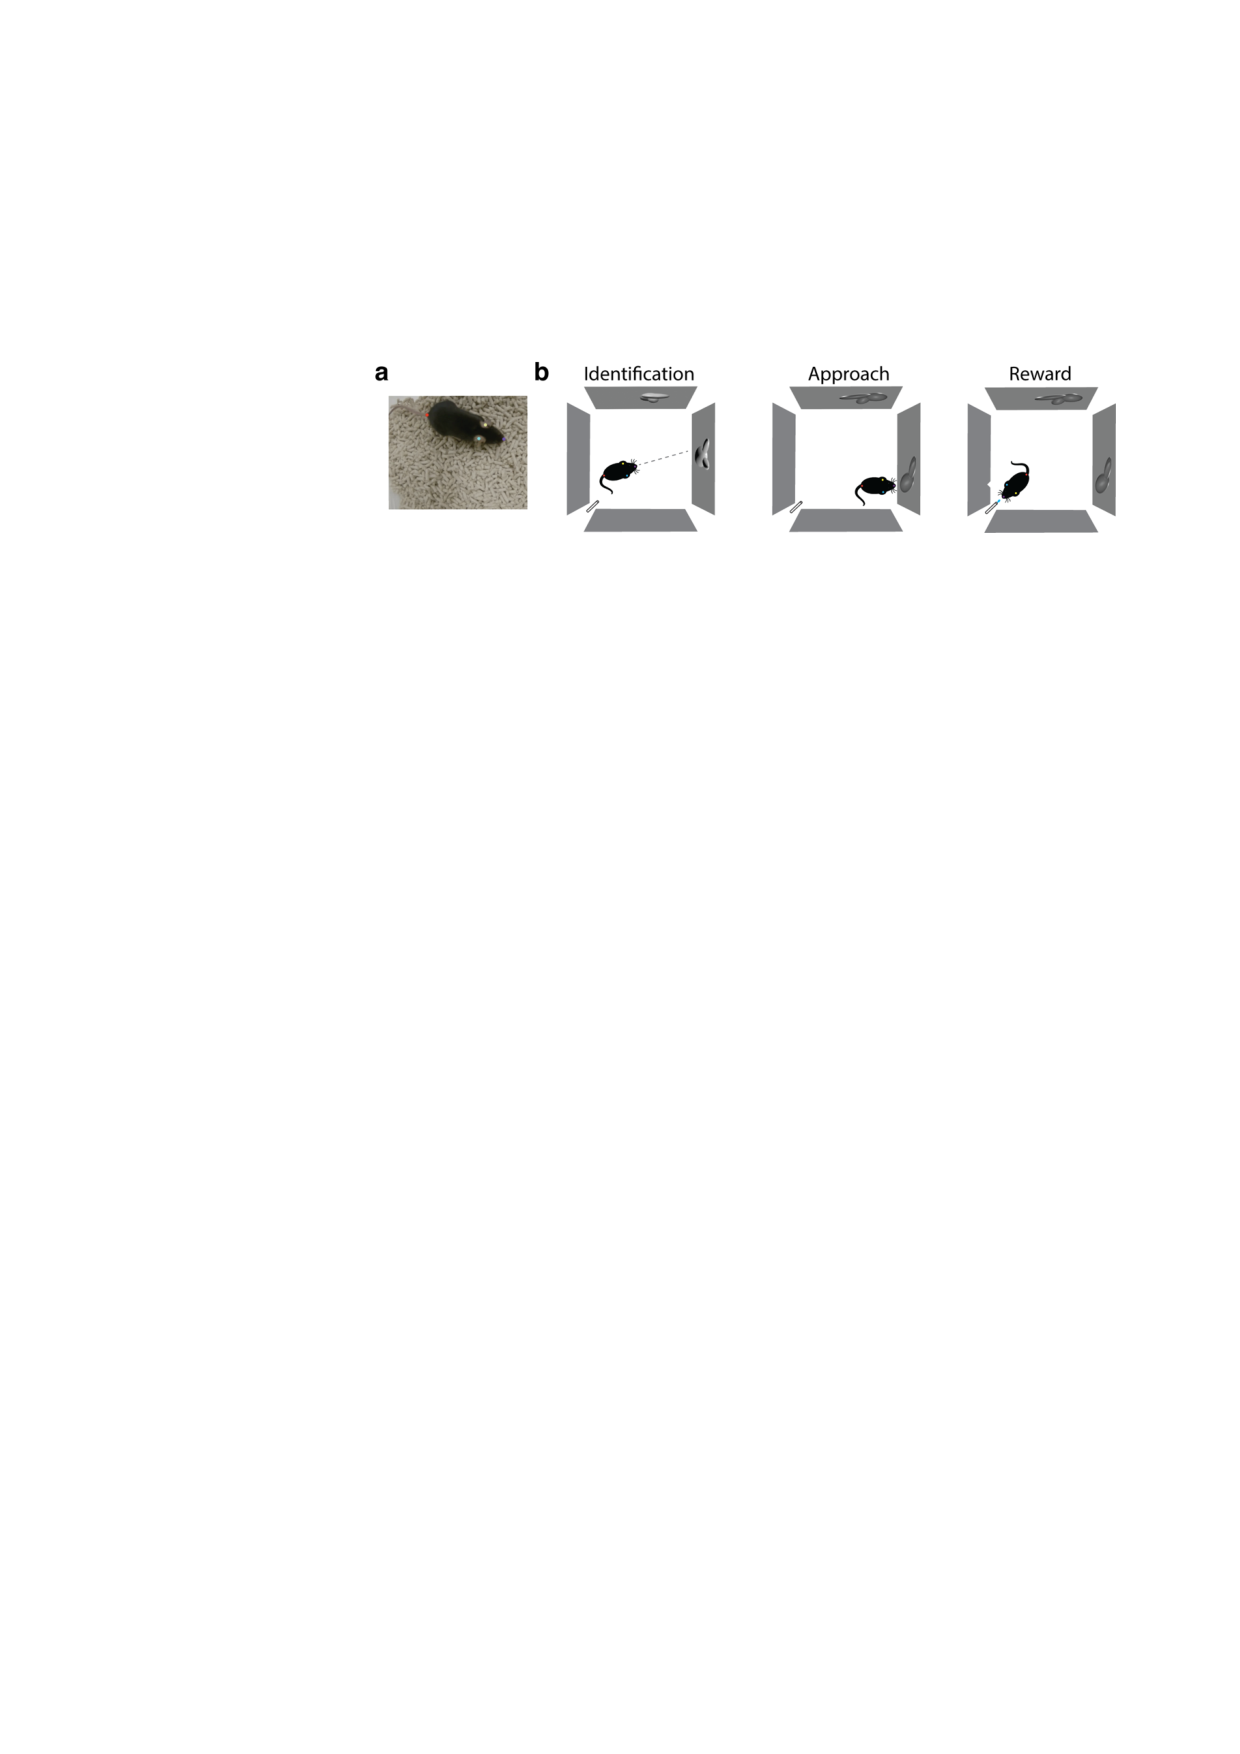
\includegraphics[width=\linewidth,trim=0 15 0 5, clip]{figures/openfield_ar.pdf}
\caption{Open field task of Dr. Froudarakis.}
\label{fig:openfield}
\end{wrapfigure}

\underline{Overview and rationale:} 
Motor behavior has been shown to strongly influence neuronal responses in head-fixed animals~\parencite{Chiappe2010-bm, Bezdudnaya2006-ge, Andermann2011-vw, Treue1996-lp,Franke2022-do, Musall2019-kd}, promising an even richer correspondence between the two in freely behaving animals. 
I will develop an approach to find correspondences between changes in stimulus selectivity and motifs of motor behavior in a data-driven way.
To quantify and interpret what these changes in tuning mean in terms of visual computation we will relate them to changes in uncertainty about semantic and geometric properties of rendered stimuli from the object recognition task and the virtual environment replica.


\underline{Approach: } 
We will use the model from \obj{1} fitted to miniscope recordings and behavioral data from freely behaving mice during an open field object recognition task (Fig.~\ref{fig:openfield}).
To get a compact description of behavior, we will build an unsupervised latent state model for behavioral motifs (\eg~running, rearing) on the posture trajectories~\parencite[similar to][]{Wiltschko2015-ey, Wiltschko2020-zd}.
This will yield a low dimensional vector for each motif that can compactly describe and generate it. 
We will then connect this with the model of~\obj{1} to obtain \texttt{neuronal activity = model(visual input, 3D posture(motif embedding))}. 
Using optimization on \texttt{motif embedding}, we will find directions in the behavior embedding space that maximally change the selectivity of a given neuron to the same stimulus.
To account for possible changes due to task context (\eg~object ID, trial state), we will include it  in the model.
To investigate my hypothesis that changes in tuning boost the reliability in specific behaviorally relevant scene aspects, we will reconstruct scene properties (such as object boundaries, curvature, slant, texture, or optical flow -- known from LIDAR scanning) under the two extreme states of stimulus selectivity. 
We will then quantify which latent scene properties change most in accuracy or uncertainty.
We will subcontract one of our experimental partners to experimentally test the properties we identified using established protocols between our labs~\parencite[used in \eg][]{Walker2019-yw, Franke2022-do}.

\underline{Expected outcome: } I expect to find changes in selectivity that are linked to specific behavioral contexts, such as enhanced object boundaries or non-self-induced optic flow during running.


%---------------------------------------------------------------------------------
\subsubsection{Objective 3: Identify causal links between neuronal representations and behavior~(4 yrs, PD, contributions from PhD1 \& PhD2)\hfill\obj{3}}
\labelobj{3}
\underline{Goal:} Use reinforcement learning to predict how the animal's behavior/ performance in an object recognition task would change if its visual processing did not adapt with motor behavior.

\underline{Overview and rationale:} 
Previous studies reported that modulation of sensory responses resulted in better behavioral performance \parencite{Spitzer1988-kq, Bennett2013-rk, Dadarlat2017-jw, De_Gee2022-ir}.
I thus hypothesize that selectivity-changes generally bias visual processing towards task- or behaviorally relevant signals.
The challenge in understanding the role of visual representations for behavior is to establish \textit{necessity}: Even when a particular neuronal mechanism is suppressed, the animal might still achieve the behavioral goal using alternative strategies. 
I propose to address this issue by letting the functional twin learn to solve the open field recognition task in the virtual replica under different manipulations of its visual system.  



\underline{Approach:} 
To predict behavior and performance of an animal in the open field object recognition task, we will use reinforcement learning~\parencite[RL,][]{Cobbe2021-op} to train an agent based on the functional twin (\obj{1}) and actions based on behavioral motifs (\obj{2}) in the virtual environment to solve the object recognition task.
We will develop the framework in stages of increasing complexity.
We will first model task decisions of head-fixed mice, where the RL-action space is limited, 
then decisions of mice in open field task for experimentally observed behavior, and finally both decisions and behavior. 
Likewise, we will first model the effect of actually performed optogenetic manipulations before moving to disabling behavior-associated changes in stimulus selectivity in the model. 
To reflect the effect of optogenetic changes we will fine tune the model on recorded data under these manipulations. 
The difference in behavior of the agent between the natural and manipulated state will make a prediction about how the animal uses these neuronal mechanisms during free behavior.
Prediction quality will be determined by how well a classifier can separate behavior of real trials from the one predicted by RL. 


\underline{Expected outcome:} 
Specific predictions about the effect of shutting down  behavior-associated changes in selectivity on task performance and behavior. 
I expect it to mostly affect behavior/performance when their associated behavioral motifs are actively used in the task.
For instance, the agent could stall while approaching the object to trade off the loss in reliability with longer observation times. 


\subsection{Risk Management}
All single parts for~\obj{1} have been previously  implemented by us~\parencite{Sinz2018-sk, Bashiri2021-or} or others~\parencite{Parker2022-ac,Holmgren2021-jv}. 
Using a forward facing and an eye camera, \textcite{Parker2022-ac} already accounted for eye movements and mapped receptive fields in behaving mice. 
However, their simple model would be insufficient for  for all objectives discussed here.
Additional risk hedging derives from the two contributions of this proposal: developing the computational framework and investigating changes in visual processing during free behavior.
For the latter, there is a risk that my hypothesis is incorrect and we do not find novel behavior-associated selectivity-changes. 
But given the number of documented cases in head-fixed animals, even that would be an important result. 
Furthermore, this would not invalidate the impact of the developed computational framework on \textit{natural neuroscience}. 

% To de-risk the project against failure of single components, \obj{2} and \obj{3} 


% We will validate that we inferred the correct eye movements from episodes in the experiments where the animal performed a task and the eyes are visible near the lick ports. If we do not infer the correct eye movements, our experimental collaborators will place an eye-tracking camera on the mouse as has been done before~\parencite{Parker2022-ac}\hl{Would be good to derisk that better; maybe say that shifter has only minor influence on the prediction performance}.

% \hl{TODO}
% \hl{What if we cannot infer the eye movements? -> Eye tracking in Andreas data?}
% \hl{What if any of the clusterings are not meaningful?}
% \hl{Is the digitization of the environment rich enough? -> Yes, mice don't see well. }
% \hl{What about non-visual cues}
% \hl{What about binocular neurons?}
%%%%%%%%%%%%% BIBLIOGRAPHY %%%%%%%%%%%%%%%%%%%
\begin{small}
\printbibliography
\end{small}

% \renewcommand\bibsection{\subsection{\refname}}
% \begin{small}
% 	\bibliographystyle{aa}
% 	\bibliography{bibliography}
% \end{small}

%%%%%%%%%%%%% CURRICULUM VITAE %%%%%%%%%%%%%%%%%%%
\newpage
\section{Curriculum vitae}

\subsection{Personal Information: Fabian Sinz}
\begin{tabular}{p{3cm}l}
	% Last name, first name: & Sinz, Fabian \\
	Date of birth:         & 09. October 1979 (German Citizen)     \\
	Website:               & \url{https://sinzlab.org}     \\
	ORCID:                 &  \url{https://orcid.org/0000-0002-1348-9736}      \\
	% Address:               & Campus Institute Data Science \\
	%                        & Goldschmidtstrasse 1    \\
	%                        & 37077 Göttingen, Germany     \\
	% Nationality:           & German      \\
        Google Scholar:         & \url{https://scholar.google.com/citations?user=xpwMxy8AAAAJ&hl=en&oi=ao}\\
        H-index  & 26 (3586 citations)
\end{tabular}

\subsection{Education}
\begin{tabular}{p{3cm}p{12cm}}
	2012
	 & \textbf{Ph.D. in Computational Neuroscience}, Graduate School of Neural and Behavioral Science, International Max Planck Research School, University of Tübingen, Germany, \underline{PhD Supervisor: Matthias Bethge}\\
    2007 & \textbf{Diploma in Bioinformatics}, University of Tübingen, Germany
\end{tabular}

\subsection{Current Position}
\begin{tabular}{p{3cm}p{12cm}}
    2021 -- 
	 & \textbf{Full Professor of Machine Learning}, 
       Campus Institute Data Science \& Institute of Computer Science,
       University of Göttingen, Germany\\
    2018 -- 2023
      & \textbf{Independent Group Leader}, 
       % Institute of Computer Science 
       University of Tübingen, Germany\\
    2018 -- 
      & \textbf{Adjunct Assistant Professor},
       Center for Neuroscience and Artificial Intelligence,
       Baylor College of Medicine, Houston, Texas, USA
\end{tabular}

\subsection{Previous Positions}
\begin{tabular}{p{3cm}p{12cm}}
    2018 -- 
      & \textbf{Research Assistant Professor},
       Center for Neuroscience and Artificial Intelligence, 
       Baylor College of Medicine, Houston, Texas, USA\\
    2015 -- 2018 
      & \textbf{Postdoctoral Associate},
       Center for Neuroscience and Artificial Intelligence,
       Baylor College of Medicine, Houston, Texas, USA\\
    2012 -- 2015 
      & \textbf{Postdoc},
       Dept. for Neuroethology, 
       University of Tübingen, Germany\\
    2007 -- 2012 
      & \textbf{Ph.D. student in Computational Neuroscience}, Max Planck Institute for Biological Cybernetics, Tübingen, Germany\\
\end{tabular}
\color{black}

\subsection{Fellowships and Awards}
\begin{tabular}{p{3cm}p{12cm}}
2019 & AWS Machine Learning Research Award, Amazon\\
2013 & Society of General Physiologists, MBL Scholarship Award\\
2006 & Best paper award, International Conference on Machine Learning\\
2013 & MBL scholarship, Marine Biological Laboratories
  scholarship for {\em Neural Systems and Behavior} (independent of the above award)\\
2008 -- 2010 & Ph.D. scholarship, German National Academic Foundation
\end{tabular}

\subsection{Supervision Of Graduate Students And Postdoctoral Fellows}
\begin{tabular}{p{3cm}p{12cm}}
2018 -- 2021 & 1 Postdoc: Edgar Y. Walker, Ph.D. (now Assistant Prof. at University of Washington, Seattle)\\
2019 -- & 4 Ph.D. students: Konstantin-Klemens Lurz, Konstantin Willeke, Mohammad Bashiri, Arne Nix\\
2021 -- & 2 Ph.D. students: Suhas Shrinivasan, Pawel Pierzchlewicz\\
2022 -- & 2 Ph.D. students: Dominik Becker, Pavithra Elumalai
\end{tabular}

\subsection{Teaching Activities}
\begin{tabular}{p{3.5cm}p{11.5cm}}
2021 --  & Probabilistic Machine Learning (2x, with Dr. Johannes Söding), Data Science (2x), Challenges and Perspectives in Neural Data Sciences (2x, lecture series, organizer), Seminar Current Topics in Machine Learning (1x, seminar), University Göttingen\\
% 2022 -- & , University Göttingen\\
2019 & Seminar on Causal Inference, Graduate School for Neural Information Processing, University Tübingen \\
2014, 2015, 2017  & G-Node Short Course on Neural Data Analysis, German Neuroinformatics Node, Ludwig Maximilian University Munich\\
% 2015 & 7th G-Node Winter Course on Neural Data Analysis, German Neuroinformatics Node, Ludwig Maximilian University of Munich\\
2014 -- 2015 &  Scientific Computing, University T\"ubingen\\
2012 -- 2015 & Essential Statistics (3x), University T\"ubingen \\
% 2014 & 6th G-Node Winter Course on Neural Data Analysis, German Neuroinformatics Node, Ludwig Maximilian University of Munich\\
2012 -- 2014 & Models of Neuronal Systems, University T\"ubingen\\
2007 -- 2010 & Essential Mathematics for Neuroscience (3x), University T\"ubingen\\
2006 & Ethics for Computer Scientists, University T\"ubingen, Seminar\\
2004 & Machine Learning and Neuroscience, University T\"ubingen, Seminar\\ 
% 2002 & Practical  Course on Technical Computer Science, University of T\"ubingen (as teaching assistant)
\end{tabular}

\subsection{Organization of Scientific Meetings}
\begin{tabular}{p{3cm}p{12cm}}
2022 & \url{https://sensorium2022.net} competition at NeurIPS 2022\\
2018, 2019  & Workshop ``Deep Learning in Computational Neuroscience'' (2x), Bernstein Conference for Computational Neuroscience, Berlin, Germany\\
2017 & 8th G-Node Short Course on Neural Data Analysis, German Neuroinformatics Node, Ludwig Maximilian University of Munich\\
\end{tabular}


\subsection{Institutional Responsibilities}
\begin{tabular}{p{3cm}p{12cm}}
2022 -- & Deputy Board Member, Campus Institute Data Science, U. Göttingen\\
2022 -- & Anti-Discrimination Commission, University Göttingen\\
2021 -- & Habilitation (Full) \& Study (Deputy) Commission, University Göttingen\\
% 2021 -- & Study Commission (Deputy Member), University Göttingen\\
2021 -- & Coordinator: BSc Program Applied Data Science, University Göttingen\\
2021-- & Equal Opportunity Representative, CRC 1233, University T{\"u}bingen\\
2019 -- 2023 & Founding Member, Institute for Bioinformatics and Medical Informatics (IBMI), University T{\"u}bingen \\
% 2018-- & Faculty Member, International Max Planck Research School for Intelligent Systems, T{\"u}bingen\\
% 2012 -- 2015 & Faculty Member, International Max Planck Research School for Neural and Behavioural Sciences, University T{\"u}bingen\\
% 2011 -- 2012 & Student Representative, Graduate School for Neural Information Processing, University T{\"u}bingen
\end{tabular}

\subsection{Reviewing Activities}
\begin{tabular}{p{3cm}p{12cm}}
Journals & Journal of Neuroscience; PLoS Computational Biology; Vision Research; Journal of Vision; Annals of Applied Statistics; Journal of Machine Learning Research; Pattern Recognition; Neural Computation; IEEE Pattern Analysis and Machine Intelligence; IEEE Transactions on Systems, Man, and Cybernetics – Part B; IEEE Transactions on Neural Networks and Learning Systems; Advances in Statistical Analysis (AStA); Machine Learning; eLife; Apidologie; Nat. Machine Intelligence\\
Conferences & CoSyNe; NeurIPS; AAAI; ICML; AIStats\\
Funding Agency & EU ERC; German Research Foundation (DFG); Alexander von Humboldt Foundation\\
\end{tabular}

\subsection{Memberships of Scientific Societies}
Member of the European Laboratory for Learning and Intelligent Systems (ELLIS); Bernstein Network for Computational Neuroscience
% \begin{itemize}
%     \item Member of the European Laboratory for Learning and Intelligent Systems (ELLIS)
%     \item Bernstein Network for Computational Neuroscience
%     % \item SMART Start Training Program for Computational Neuroscience, Bernstein Network and Volkswagen Stiftung (faculty)
%     % \item International Max Planck Research School for Intelligent Systems (faculty)
%     % \item Excellence Cluster Machine Learning in Science, University T{\"u}bingen
%     % \item Bernstein Center for Computational Neuroscience, Universities T{\"u}bingen \& Göttingen
%     % \item Tübingen AI Competence Center, Member
%     % \item Göttingen AI Service Center (KISSKI)
% \end{itemize}

\subsection{Major Collaborations}
Andreas Tolias \& Katrin Franke (Baylor College of Medicine, Houston); ‪‪Emmanouil Froudarakis (FORTH, Crete); Kathrin Brockmann (Hertie Institute for Clinical Brain Science, Tübingen); Leif Saager (University Hospital Göttingen); Alexander Gail (German Primate Center, Göttingen) 
% \subsection{Career Breaks}
% \subsection{Covid-19 Impact to Scientific Productivity}
% \begin{itemize}
    % \item 
% \end{itemize}

%%%%%%%%%%%%% APPENDIX %%%%%%%%%%%%%%%%%%%
\newpage
\section*{Appendix:\\ All ongoing and submitted grants and funding of the PI (Funding ID)}
\subsection{On-going Grants}
\begin{footnotesize}
	\def\arraystretch{1.5}
	\begin{tabular}{|p{3.9cm}|p{2.5cm}|p{1.5cm}|p{1.3cm}|p{1.8cm}|p{2.4cm}|}
		\hline
		\rowcolor{black!20}
		\textbf{Project Title}         &
		\textbf{Funding source}        &
		\textbf{Amount\newline(Euros)} &
		\textbf{Period}                &
		\textbf{Role of the PI}        &
		\textbf{Relation to \newline current ERC \newline proposal}          \\
		\hline
		Mechanisms of Representation Transfer  
            & CyberValley Research Fund 
            & \EUR{204,000} 
            & 10/2019 -- 09/2023 
            & PI 
            & None \\
		\hline
		KI-basiertes Tracking-System zur automatisierten, objektiven und reproduzierbaren Durchführung von Verhaltensstudien an Maus-Modellen zur Erforschung des Epilepsie- Spektrums (KI-Track)  
        & Federal Ministry for Economic Affairs and Climate Action 
        & \EUR{188,062} 
        & 10/2019 -- 04/2024 
        & PI 
        & Develops methods for 2D-3D pose lifting and \textit{supervised} action classification in mice (used in the proposal)\\
		\hline
	A collaborative data management platform for reproducible neuroscience and machine learning 
        & German Research Foundation: CRC 1233 ``Robust Vision'', University Tübingen
        &\EUR{242,700} (own part) & 01/2020 -- 12/2024 
        & Co-PI with Philipp Berens, University Hospital Tübingen & None \\\hline
    	Top-down control of visual inference in sensory representations in early visual cortex 
        & German Research Foundation: CRC 1233 ``Robust Vision'', University Tübingen &\EUR{213,020} (own part) & 01/2020 -- 12/2024 & Co-PI with Jakob Macke & Develops trainable normative models for macaque V1 \\\hline
        Predictive models and frame of reference in macaque sensorimotor cortex under natural conditions	
        & German Research Foundation: CRC 1456 ``Mathematics of Experiment'', University Göttingen
        &  \EUR{145,400} (own part) 
        & 01/2023 -- 12/2024
        & Co-PI with Alexander Gail, German Primate Center
        & Develops graph based predictive models for the sensorimotor system of macaques \\\hline
	Predicting clinical progression in Parkinson's disease patients using genetic and cerebrospinal fluid-based biomarkers. 
        & ClinBrAIn Else Kröner Medical Scientist Kollegs 
        &  \EUR{75,000} (own part)
        & 01/2023 -- 12/2025 
        & Co-PI with Kathrin Brockmann, Hertie Institute for Clinical Brain Science 
        & None \\\hline
	Inception loops for interpretable tuning in macaque area V4 
        & Collaborative Research in Computational Neuroscience (CRCNS; National Science Foundation and Federal Ministry of Education and Research) 
        &  \EUR{275,774} (own part)
        & 07/2022 -- 06/2025 
        & Co-PI with Andreas Tolias, Baylor College of Medicine 
        & Develops predictive models for macaque V4 under free viewing \\\hline
	\end{tabular}

	\begin{tabular}{|p{3.9cm}|p{2.5cm}|p{1.5cm}|p{1.3cm}|p{1.8cm}|p{2.4cm}|}
		\hline
		\rowcolor{black!20}
		\textbf{Project Title}         &
		\textbf{Funding source}        &
		\textbf{Amount\newline(Euros)} &
		\textbf{Period}                &
		\textbf{Role of the PI}        &
		\textbf{Relation to \newline current ERC \newline proposal}          \\
		\hline      
        Lung protective ventilation & University Göttingen Intramural Funding 
        & \EUR{10,157} (own part) 
        & 01/2023 -- 12/2023 
        & Co-PI with Anne-Christin Hauschild, University Hospital Göttingen
        & None\\\hline
        KI-EIT: Evaluation des Potenzials künstlicher Intelligenz (KI) zur Erfassung von beginnenden Lungengewebsschädigungen mittels Elektrischer Impedanztomographie (EIT) durch Langzeitmonitoring
        & German Aerospace Center
        & \EUR{253,509} (own part)
        & 11/2022-10/2025 
        & Co-PI with Leif Saager, University Hospital Göttingen
        & None\\\hline
	\end{tabular}
\end{footnotesize}
\color{black}

\subsection{Applications}
\begin{footnotesize}
	\def\arraystretch{1.5}
	\begin{tabular}{|p{3.9cm}|p{2.5cm}|p{1.5cm}|p{1.3cm}|p{1.8cm}|p{2.4cm}|}
		\hline
		\rowcolor{black!20}
		\textbf{Project Title}         &
		\textbf{Funding source}        &
		\textbf{Amount\newline(Euros)} &
		\textbf{Period}                &
		\textbf{Role of the PI}        &
		\textbf{Relation to \newline current ERC \newline proposal}          \\
		\hline
		Mechanistic dissection of ethological visual inference during prey capture                           & National Institute of Health (NIH) U19 & \EUR{491,382} (own part) & 2023-2027 & Co-Investigator on Project 3 & Proposes to study visual representations along mouse cortical hierarchy during hunting (some of the data could be used for the ERC, but methods/goals are different)\\
		\hline
		Brain CoLaboratory: Accelerating scientific discovery though a community effort using inception loops
        & National Institute of Health (NIH) U24 
        & \EUR{676,912} (own part) 
        & 2023-2027 & Co-Investigator with Andreas Tolias, Baylor College of Medicine
        & None\\
		\hline
	Curiosity
        & Research Training Center, German Research Foundation
        & \EUR{454,600} (own part) 
        & 2024-2029 & Co-PI with Nivedita Mani, University Göttingen
        & None\\
		\hline
        Identifying molecular endophenotypes and clinical PD subtypes by modelling demographic, lifestyle, genetic and CSF biomarker signatures 
        & Michael J. Fox Foundation
        & \EUR{126,410} (own part) 
        & 2023-2026 & Co-PI with Kathrin Brockmann, Hertie Institute for Clinical Brain Research
        & None\\
		\hline
	\end{tabular}
\end{footnotesize}

%%%%%%%%%%%%% APPENDIX %%%%%%%%%%%%%%%%%%%
\newpage
\section{Early achievements track-record}
\label{sec:trackrecord}
\subsection{Highlights}
\begin{itemize}
    \item Raised more than \EUR{1.8M} in third party funding (counting own share only).
    \item $>70$ peer reviewed publications and preprints on machine learning and neuroscience published in high ranking journals and top tier conferences: $>$3500 citations, h-index 26 (google scholar), 8 publications from my undergraduate work (6 conference, 1 journal, 1 book chapter).
    \item Best paper award (2nd author) at ICML 2006 (top tier conference).
    \item Since the start of my own lab in late 2018: Over 20 peer reviewed paper in top tier conferences (\textit{i.a.} NeurIPS, ICLR) and high impact journals (\textit{i.a.} Nature, Nature Neuroscience, Nature Communications, Neuron), and over 10 preprints; 7 journal, 10  conference, 5 workshop, 13 preprints.
    \item In executive leadership team (machine learning coordinator, 2016--2021) of \$20M \href{https://www.ninai.org/}{international consortium (MICrONS)} of multiple research institutions (\textit{i.a.} Baylor College of Medicine, Princeton, CalTech, Columbia, Allen Institute, Vector Institute/U Toronto) to understand algorithms of vision.
    \item Independent Group Leader at Europe's largest AI research consortium (\href{https://cyber-valley.de/}{CyberValley}).
    \item Tenured full professor and institute board member. 
\end{itemize}

\subsection{Scientific independence, interdisciplinarity, and leadership}
Throughout my career, I have always strived for scientific independence and breadth. Even before I obtained my diploma (master's degree), I independently worked on my own  projects as a student assistant at the Max Planck Institute for Biological Cybernetics in the department of Bernhard Schölkopf and as an intern at NEC research in Princeton. My undergraduate work resulted in eight publications, one of them a best paper award at the top tier International Conference for Machine Learning (ICML) and one of them with one of the fathers of statistical machine learning (Vladimir Vapnik). During my time as a graduate student, I secured my own funding through a Ph.D. scholarship, independently started multiple collaborations (\eg~with HHMI investigator Eero Simoncelli), and taught my own lectures for master students. My graduate work resulted in nine publications, seven of them as first author. 

My scientific passion is to understand the building blocks of biological intelligence, using computational tools from artificial intelligence. After my Ph.D., I thus decided to do some experimental neuroscience work as a postdoc. I first spent three years in an electric fish lab until I joint the lab of Andreas Tolias in Houston where I got the opportunity to join both of my interests in a large multi-university consortium (MICrONs). I quickly became part of the executive leadership team (machine learning coordinator), where I made several key conceptual contributions that led our consortium to be the only one (out of three) that made it through all three funding phases (consortia led by Harvard and CMU were eliminated earlier). Subsequently, I became a research assistant professor at Baylor College of Medicine in Houston in 2018, an independent group leader in Europe's largest consortium for AI research  (\href{https://cyber-valley.de/}{CyberValley}) in 2018, before accepting a full W3 professorship in Göttingen (2021).

The focus of my research group today is developing machine learning models for complex life science data, in particular neuroscience. We draw great scientific satisfaction from compiling multiple experimental datasets into predictive models (functional digital twins) that can make predictions which would have been infeasible to find experimentally, but that can be verified experimentally (\eg~because searching is hard in experiments, but feasible in computational models). For that, we are very fortunate to closely work with experimentalists (A. Tolias \& K. Franke in Houston, E. Froudarakis on Crete, A. Gail in Göttingen) who trust us with their data and run the verification experiments.

\subsection{Selected publications as (joint$^{\color{red}\fstar}$) senior author (none with Ph.D. supervisor)}
\begin{itemize}[topsep=0pt,itemsep=0.62ex,partopsep=0ex,parsep=0.5ex]
    \item Franke K, Willeke KF, Ponder K, Galdamez M, Muhammad T, Patel S, Froudarakis E, Reimer J, \textbf{Sinz FH}$^{\color{red}\fstar}$, Tolias AS$^{\color{red}\fstar}$ (2022). \textit{Behavioral state tunes mouse vision to ethological features through pupil dilation}. \textbf{Nature}. \href{https://www.nature.com/articles/s41586-022-05270-3}{Link}
    
    $\rightarrow$~\textit{Joint last authorship (computational PI). Uses functional digital twins combined with experiments to show that color tuning can change in mouse visual cortex on the order of seconds. }
    
    \item Bashiri M, Walker EY, Lurz KK, Jagadish AK, Muhammad T, Ding Z, Ding Z, Tolias AS, \textbf{Sinz FH} (2021). \textit{A flow-based latent state generative model of neural population responses to natural images} \textbf{NeurIPS}. \href{https://openreview.net/forum?id=1yeYYtLqq7K}{Link}
    
    $\rightarrow$~\textit{First full image driven neuronal encoding model with latent state for thousands of neurons from multiple areas. Selected as spotlight. NeurIPS is the top tier machine learning conference (2021: 25.8\% acceptance rate, 12\% spotlight)}.
    
    \item Lurz KK, Bashiri M, Willeke KF, Jagadish AK, Wang E, Walker EY, Cadena S, Muhammad T, Cobos E, Tolias AS, Ecker AS, \textbf{Sinz FH} (2021) \textit{Generalization in data-driven models of primary visual cortex.} \textbf{ICLR}. \href{https://openreview.net/forum?id=Tp7kI90Htd}{Link}
    
    $\rightarrow$~\textit{First paper to demonstrate that data-driven models of mouse visual cortex learn characteristic features that generalize between animals. De-facto state of the art model for neural prediction in mouse visual cortex. Selected as spotlight at ICLR. ICLR is among the top-tier conferences for machine learning (2021: 28.7\% acceptance rate, 3\% spotlight)}.
\end{itemize}

\subsection{Selected publications as (joint$^{\color{red}\fstar}$) first author (none with Ph.D. supervisor)}
\begin{itemize}[topsep=0pt,itemsep=0.62ex,partopsep=0ex,parsep=0.5ex]
    \item Walker EY$^{\color{red}\fstar}$, \textbf{Sinz FH}$^{\color{red}\fstar}$, Cobos E, Muhammad T,  Froudarakis E, Fahey PG, Ecker AS, Reimer J, Pitkow X, Tolias AS (2019) \textit{Inception loops discover what excites neurons most using deep predictive models} \textbf{Nature Neuroscience}. \href{https://www.nature.com/articles/s41593-019-0517-x}{Link}

    $\rightarrow$~\textit{One of the three first papers to show that data-driven functional digital twin models can be used to derive novel insights about single neurons in visual cortex. Two similar papers (\href{https://www.science.org/doi/10.1126/science.aav9436}{Bashivan et al. 2019}, \href{https://www.sciencedirect.com/science/article/pii/S0092867419303915}{Ponce et al. 2019}) were published concurrently}.
 
    \item \textbf{Sinz FH}, Ecker AS, Fahey PG, Walker EY, Cobos E, Froudarakis E, Yatsenko D, Pitkow X, Reimer J, Tolias AS (2018) \textit{Stimulus domain transfer in recurrent models for large scale cortical population prediction on video}. \textbf{NeurIPS}. \href{https://proceedings.neurips.cc/paper/2018/file/9d684c589d67031a627ad33d59db65e5-Paper.pdf}{Link}

    $\rightarrow$~\textit{First deep learning based functional digital twin model for visual cortex on video. Reproduces tuning properties of single neurons when trained on natural videos only. NeurIPS is the top tier conference in machine learning (2018: acceptance rate 20.8\%)}.
\end{itemize}


\subsection{Scientific achievements}
\begin{itemize}[topsep=0pt,itemsep=0.62ex,partopsep=0ex,parsep=0.5ex]
    \item I am the co-developer of the \textit{Inception Loop} method (Walker, Sinz et al., 2019) that uses deep learning models to learn a functional copy of a neural system from responses to natural stimuli, to derive predictions \textit{in silico} (such as optimal stimuli) and to verify them \textit{in vivo}. This method is an effective way to circumvent many experimental difficulties by ``outsourcing'' searching (for best stimuli, invariances, etc.) to a computational model.    
    Using inception loops, we (computationally and experimentally) demonstrated striking deviations of mouse primary visual cortex from existing textbook models (Walker, Sinz et al., 2019), and showed that visual cortex can change selectivity with behavioral states on the order of seconds (Franke et al, 2022).
    \item I pioneered scalable data-driven deep learning models of the primary visual cortex on video (Sinz et al., 2018) and deep latent (brain) state models that can be driven by arbitrary images (Bashiri et al., 2021). These models are trained on responses to natural images and extrapolate non-trivially to meaningful properties of the real neurons, such as direction tuning or brain area membership. These models form the basis for the work proposed here.  
    \item During my Ph.D. I derived novel parametric distributions for natural images (Sinz, Bethge, 2010; Sinz, Simoncelli, Bethge, 2009) that were state of the art at the time, and derived a non-trivial characterization of the Gaussian distribution to non-Euclidean norms (Sinz, Gerwinn, Bethge, 2009). The original result for Gaussians is attributed to Maxwell.
\end{itemize}


% \subsection{Talks}
% \subsubsection{\textit{Selected Colloquia}}

% \begin{longtable}{p{7.5cm}p{6cm}l}
% 	Seminar & A University & date \\
% 	Seminar & B University & date \\
% \end{longtable}

% \subsection{\textit{Selected Conference Talks}}

% \begin{longtable}{p{7.5cm}p{6cm}l}
% 	Invited review on Blabla & City & date \\
% \end{longtable}

\end{document}
